\section{Information Theory}%
\label{sec:information-theory}

\vspace{1cm}

\begin{figure}[h]%
  \label{fig:info}
  \centering
  \fcolorbox{black}{white}{\includegraphics[width=0.3\textwidth]{entropy}}
  \caption{\href{https://www.consciousentities.com/2017/02/consciousness-entropy/}{Conscious
      Entities, Peter Hankins}}
\end{figure}

\vspace{1cm}

\lettrine[lines=3]{\Royal~I} {nformation theory was born in 1948 with
  the publication} of \textit{A Mathematical Theory of Communication}
by Claude Shannon (1916~\textendash~2001). Shannon's work was inspired
in part by earlier work by Ludwig Boltzmann and Josiah Willard Gibbs
in the theory of thermodynamics. Most of the theory and applications
of information theory (compression, coding schemes, data transfer over
noisy channels) are outside the scope of this paper, but there are
certain information theoretic quantities used regularly in machine
learning, so it is useful to discuss them now.

\begin{remark}
  The information we talk about is restricted to the information about
  the probability distribution over the events, not information about
  the events themselves.

  The significance of probability is that it tells us when we can be
  certain about making inference. The most important information in
  this regard is found in the probability distribution over the
  possible events. When the distribution is uniform, we can't really
  make any inference.
\end{remark}

Information theory is quite useful for deep learning. If we think of
neural nets as noisy channels, the need for this theory becomes even
more obvious. In~\cite{ref:mackay-2003}, David Mackay said ``brains
are the ultimate compression and communication systems. And the
state-of-the-art algorithms for both data compression and
error-correcting codes use the same tools as machine
learning''. Furthermore, ``we might anticipate that the best data
compression algorithms will result from the development of artificial
intelligence methods''.

The most fundamental quantity in information theory is
\textit{entropy}. Before we state the formal definition of entropy, we
will motivate it as a measure of \textit{uncertainty} by walking
through its derivation. We will define a function $\eta$ as a measure
of uncertainty. We will derive entropy as a function based on the
requirements it must satisfy.

\begin{definition}
  Let $(\&X, p(x))$ be a finite probability space. We define
  \textbf{uncertainty} to be a real-valued function $\eta(\cdot): \&X \mapsto
  \R^+$ which depends only on the probabilities of the events and satisfies the
  following:
  \begin{enumerate}[(i)]
  \item If an event $x$ is guaranteed to occur, then there is no uncertainty
    about it and $\eta(x) = 0$;
  \item For any two events $x$, $x^\prime$, we have $p(x) < p(x^\prime) \iff
    \eta(x) > \eta(x^\prime)$;
  \item For any two events, $x$, $x^\prime$, the uncertainty of their
    simultaneous occurrence, is the sum of their uncertainties, i.e. $\eta(x
    \cdot x^\prime) = \eta(x) + \eta(x^\prime)$.
  \end{enumerate}
\end{definition}
\begin{remark}
  This definition is a modification of one given by~\cite{ref:martin-2011}.
\end{remark}

It shouldn't be a surprise that it's new information we are interested in, since
that is what reduces uncertainty. Common events provide less information than
rare events, which means $\eta$ should be inversely proportional to the
probability of the event.
\begin{align}
  \label{eq:eta-1}
  \eta(x) \propto {1 \over p(x)}
\end{align}
Thus, $\eta$ should be maximized when we cannot say with any confidence if an
event will occur. This upper bound should occur when the probabilities over the
set of possible events are uniformly distributed.
\begin{align}
  \label{eq:eta-2}
  \eta(x) \leq {1 \over |\&X|}
\end{align}
Since $\eta$ must satisfy $\eta(x \cdot x^\prime) = \eta(x) + \eta(x^\prime)$,
we must define $\eta$ in terms of the logarithm, which provides additivity where
once was only multiplicity.
\begin{align}
  \label{eq:eta-3}
  \eta(x) \approx \log{\left({1 \over p(x)}\right)}
\end{align}
Where the logarithm is to the base 2. For probability distributions not equal to
the uniform distribution, we need a more precise estimate of measuring how much
uncertainty, \textit{on average}, is contained in events from $(\&X, p(x))$. We
need to weight the calculation by the probability of observing each event. This
means what we are really seeking is a measure on the probability distribution
over $\&X$, since that is where the information about the probability of events
is stored. We will adjust the notation, we wil use the upper case of $\eta$,
which resembles the Latin H,
\begin{align}
  \label{eq:eta-almost}
  \&H(P) = \sum_{x \in \&X} p(x) \log\left({1 \over p(x)}\right).
\end{align}
This is what we will call entropy, a measures on the average amount of surprise
associated with events from $(\&X, p(x))$. We can also think of it as, how much
information, measured in \textit{binary information units} (bits), is required
to describe events drawn from $(\&X, p(x))$. The way to understand this last
part is the logarithm tells us how many bits we need to describe this
uncertainty, since
\begin{align}
  \label{eq:understand-log}
  \log_2\left( {1 \over p(x)} \right) = n \iff 2^n = {1 \over p(x)}.
\end{align}
\begin{definition}
  The \textbf{entropy} of a probability distribution $P$ with mass function
  $p(x)$, denoted by $\&H(P)$, is the average number of bits required to
  describe individual samples drawn from $\&X$ under $p(x)$. We write
  \begin{align}
    \label{eq:entropy}
    \&H(P) = - \mathbb{E}_{x \sim p(x)} \left[ \log{p(x)} \right].
  \end{align}
  The entropy of a probability distribution tells us how much variation we
  should expect to see in samples drawn from $(\&X, p(x))$. It as a measure of
  uncertainty and surprise. The probability distribution with maximum entropy is
  the uniform distribution since all events are equally surprising.
\end{definition}

Figure \ref{fig:entropy-coin-toss} depicts the entropy of a probability
distribution over two states as a function of the symmetry of the distribution.
As the probability of heads $p(H)$ approaches 0 or 1, we see the uncertainty
vanishes, and uncertainty is maximized when probability is equally distributed over heads and tails.

\begin{figure}[H]
  \centering
  \begin{tikzpicture}
    \begin{axis}[
      ymin = 0,
      ymax = 1,
      xmin = 0,
      xmax = 1,
      xlabel = $p(H)$,
      ylabel = $\&H(P)$,
      enlargelimits = false]
      \addplot [samples = 300, blue] {-x*log2(x)-(1-x)*log2(1-x)};
    \end{axis}
  \end{tikzpicture}
  \caption{Entropy of a coin toss as a function of the symmetry of $p(H)$.}
  \label{fig:entropy-coin-toss}
\end{figure}

\begin{example}
  The entropy of the probability distribution corresponding to a fair coin toss
  is 1 bit, and the entropy of $m$ tosses is $m$ bits. If there are two states
  of equal probability, then we need 1 bit and if we have 3 states of equal
  probability, we need 1.584963 bits.
\end{example}

We include a definition of a \textit{metric} below in order to make make clear
the distinction between it and a \textit{divergence}, which will be define
afterwards.

\begin{definition}
  A \textbf{metric} on a set $\&X$ is a function $d(\cdot, \cdot): \&X \times
  \&X \mapsto \R^+$ such that, $\forall x, y, z \in \&X$:
  \begin{enumerate}
  \item $d(x, y) \geq 0$
  \item $d(x, y) = 0 \iff x = y$
  \item $d(x, y) = d(y, x)$
  \item $d(x, z) \leq d(x, y) + d(y, z)$
  \end{enumerate}
\end{definition}

\begin{remark}
  A \textit{divergence} is a weaker notion than that of distance. A divergence
  need not be symmetric nor satisfy the triangle inequality.
\end{remark}

\begin{definition}
  Let $\&P$ be any space of probability distributions over any finite set such
  that all
  $P \in \&P$ have the same support. A \textbf{divergence} on $\&P$ is a
  function, $\&D\left( \cdot \mid\mid \cdot \right): \&P \times \&P \mapsto
  \R^+$, such that $\forall P, Q \in \&P$ the following conditions are
  satisfied
  \begin{enumerate}[(i)]
  \item $\&D(P||Q) \geq 0$
  \item $\&D(P||Q) = 0 \iff P = Q$.
  \end{enumerate}
\end{definition}

\begin{definition}
  The \textbf{Kullback-Leibler divergence} is a measure of how one probability
  distribution is different from a second, reference probability distribution.
  It is also known by the following names, \textbf{relative entropy},
  \textbf{directed divergence}, \textbf{information gain} and
  \textbf{discrimination information}.
  \begin{align}
    \label{eq:KL}
    \KL{P}{Q} = \sum_{x \in \&X} p(x) \log{p(x) \over q(x)}.
  \end{align}
\end{definition}

The Kullback-Leibler divergence is not a metric since it is not symmetric. If
$P$ and $Q$ have the same support, then $\KL{P}{Q} = 0$ if and only if $P = Q$.

\begin{theorem}
  For a closed convex set $E \subset \&P$, where $\&P$ is the space of
  all probability distributions over a finite set $\&X$, and for a
  distribution $Q \not \in E$, let $P^* \in E$ be defined by
  $P^* = \argmin_{P \in E} \KL{P}{Q}$, then
  \begin{align}
   \KL{P^*}{Q} \geq \KL{P}{P^*} + \KL{P^*}{Q}.
  \end{align}
  The interested reader can consult Theorem 11.6.1 in~\cite{ref:cover-thomas}.
\end{theorem}

\begin{remark}
  The Kullback-Leibler divergence of $P$ and $Q$ is the average of the
  log-likelihood ratio test with respect to probabilities defined by $P$. The
  average is taken over the data points, not the parameters. The log-likelihood
  ratio test is used in comparing the goodness-of-fit of one statistical model
  over another. For two models $p(x) = f(x|\theta)$ and $q(x) = f(x|\phi)$,
  the log-likelihood ratio test is
  \begin{align}
    \lambda(x) & = \log{\prod_{x \in \&X} p(x) \over \prod_{x \in \&X} q(x)} \\
               & = \log \prod_{x \in \&X} {p(x) \over q(x)} \\
               & = \sum_{x \in \&X} \log {p(x) \over q(x)}
  \end{align}
  and the average with respect to $p(x)$ is
  \begin{align}
    \E{x \sim p(x)}{\lambda(x)} = \sum_{x \in \&X} p(x)\log {p(x) \over q(x)}.
  \end{align}
\end{remark}
The term \textit{information gain} refers to one interpretation of the
Kullback-Leibler diverence, specifically $\KL{P}{Q}$ is the amount of
information gained about the data when $Q$ is used to model the data, rather
than $P$.  Equivalently, the amount of information lost when $Q$ is used to
approximate $P$.

\begin{definition}
  The \textbf{reverse Kullback-Leibler divergence} is the asymmetrical
  counterpart.
  \begin{align}
    \label{eq:reverse-KL}
    \KL{Q}{P} = \sum_{x \in \&X} q(x) \log{q(x) \over p(x)}.
  \end{align}
  The reverse Kullback-Leibler divergence is the average of the log-likelihood
  ratio test taken with respect to the model $q(x)$,
  \begin{align}
    \E{x \sim q(x)}{\lambda(x)} = \sum_{x \in \&X} q(x)\log {q(x) \over p(x)}.
  \end{align}
\end{definition}

Minimizing the reverse Kullback-Leibler divergence is not equivalent to maximum
likelihood methods, see (\ref{eq:equivalent-mle}). The Kullback-Leibler
divergence is related to another quantity used in machine learning quite often,
\textit{cross entropy}.

\begin{definition}
  The \textit{cross entropy} of $P$ and $Q$ (for a given data set) is the total
  amount of uncertainty incurred by modelling the data with $Q$ rather than $P$.
  \begin{align}
    \&H(P,Q) = - \sum_x p(x) \log q(x) = -\mathbb{E}_{x \sim p(x)}\left[\log{q(x)}\right].
  \end{align}
\end{definition}

\begin{lemma}
The cross entropy of $P$ and $Q$ is the sum of the entropy of $P$ and the
Kullback-Leibler divergence of $P$ and $Q$.
\end{lemma}
\begin{proof}
\begin{align}
  \label{eq:cross-entropy-alt}
  \&H(P, Q) & = -\sum_{x \in \&X} p(x) \log q(x) \\
            & = -\sum_{x \in \&X} p(x) \log p(x) + \sum_{x \in \&X} p(x) \log p(x) - \sum_{x \in \&X} p(x) \log q(x) \\
            & = -\sum_{x \in \&X} p(x) \log p(x) + \sum_{x \in \&X} p(x) \log {p(x) \over q(x)} \\
            & = \&H(P) + \KL{P}{Q}
\end{align}
\end{proof}

Which tells us the lower bound for cross entropy must be the entropy of the
probability distribution $P$ over $\&X$. Thus, cross entropy is the uncertainty
induced by assuming the wrong probability distribution over the data. The
additional uncertainty is captured by the Kullback-Leibler divergence. Cross
entropy is not symmetric since $\&H(Q, P) = \&H(Q) + \KL{Q}{P}$.

One reason that GANs are so successful is because they do not rely on
traditional maximum likelihood methods (why is this so?), which are equivalent
to minimizing the Kullback-Leibler divergence. To see this, let $p\left(x |
  \theta^{(*)}\right)$ be a probability distribution we wish to estimate and let
$p\left(x | \theta^{\left(t\right)}\right)$ be our estimate at iteration $t$.
Then
\begin{align}
  \label{eq:equivalent-mle}
  \KL{p\left(x | \theta^{(*)}\right)}{p\left(x | \theta^{\left(t\right)}\right)} =
  H\left(p\left(x | \theta^{(*)}\right)\right) -
  \mathbb{E}_{x \sim p\left(x | \theta\right)}\left[ \log p\left(x | \theta^{\left(t\right)}\right) \right],
 \end{align}
 and minimizing the cross entropy term on the right is equivalent to maximizing
 \begin{align}
   \mathbb{E}_{x \sim p\left(x | \theta\right)}\left[ \log p\left(x | \theta^{\left(t\right)}\right) \right].
 \end{align}
 Maximizing this term is equivalent to maximizing the likelihood
 function for $p\left(x | \theta\right)$. Instead, as shown
 in~\cite{ref:goodfellow-original}, the generator minimizes an
 approximation of the \textit{Jensen-Shannon divergence}.

\begin{definition}
  \label{def:jsd}
  Let $p(x)$ and $q(x)$ be any two probability distributions over any space
  $\&X$. The \textit{Jenson-Shannon divergence} of $p(x)$ and $q(x)$ is a
  symmetrization of the Kullback-Leibler divergence of $p(x)$ and $q(x)$ over
  $\&X$.
  \begin{align}
    \JSD{P}{Q} = {1 \over 2} \KL{P}{P + Q \over 2} + {1 \over 2} \KL{Q}{P + Q
    \over 2}
  \end{align}
\end{definition}
\begin{remark}
  The Jensen-Shannon divergence is the average of the Kullback-Leibler
  divergence and the reverse Kullback-Leibler divergence.
\end{remark}

\begin{theorem}
  The square root of the Jensen–Shannon divergence is a metric.
\end{theorem}
\begin{proof}
  See~\cite{ref:endres-2003}.
\end{proof}

\subsubsection{Mutual Information and other Measures}

Information theory provides us with a measure of dependency, or at least how
much information about one probability distribution is contained in another
distribution.

\begin{definition}
  Let $\&X$ and $\&Y$ be any two sets (not necessarily distinct) and consider
  two random variables $X \sim P$ and $Y \sim Q$ with joint probability mass
  function $\gamma(x,y)$ and marginal probability mass functions $p(x)$ and
  $q(y)$. The \textit{mutual information} $I(X;Y)$ is the Kullback-Leibler
  divergence of $\gamma(x,y)$ and the product of $p(x)$ and $q(y)$, in other
  words
  \begin{align}
    \label{eq:mutual-information}
    \&I(X; Y) = \sum_{x \in \&X}\sum_{y \in \&Y}\gamma(x, y) \log{{\gamma(x, y) \over p(x)q(y)}}
  \end{align}
\end{definition}

\begin{theorem}
  If the random variables $X$ and $Y$ are independent, then $\gamma(x,y) = p(x)q(y)$
  and $\&I(X; Y) = 0$.
\end{theorem}

\begin{remark}
  Mutual information is a measure of the amount of information contained in one
  probability distribution about another and makes for a useful measure of
  statistical dependence.
\end{remark}

\begin{remark} Mutual information can also be defined in terms of conditional
  entropy.
  \begin{align}
    \label{eq:mutual-information-alt}
    \&I(X; Y) = \&H(X) - \&H(X \mid Y) = \&H(Y) - \&H(Y \mid X)
  \end{align}
  Where $\&H(X \mid Y)$ is the conditional entropy of $X$ given that $Y$ has
  occurred. In this form the mutual information can be interpreted as the
  information contained in one probability distribution minus the information
  contained in the distribution when the other distribution is known.
  \end{remark}

  The relationship different information theoretic quantities is depicted in the
  Venn diagram in Figure~(\ref{fig:venn-information}).

\begin{figure}[h]
  \centering
  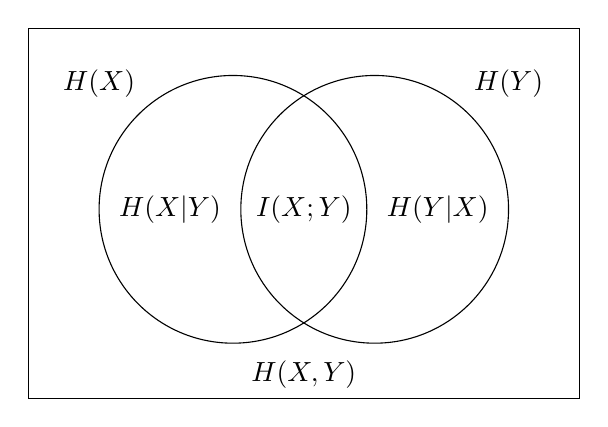
\begin{tikzpicture}
    % Labels
    \draw (0,0) node {$I(X;Y)$};
    \draw (-2.6,1.6) node {$H(X)$};
    \draw (2.6,1.6) node {$H(Y)$};
    \draw (-1.7,0) node {$H(X|Y)$};
    \draw (1.7,0) node {$H(Y|X)$};
    \draw (0,-2.1) node {$H(X,Y)$};
    % Circles
    \draw (-0.9,0) circle (1.7cm);
    \draw (0.9,0) circle (1.7cm);
    % Bounding Rectangle
    \draw (-3.5,-2.4) rectangle (3.5,2.3);
  \end{tikzpicture}
  \caption{Venn Diagram of Information-Theoretic Quantities}%
  \label{fig:venn-information}
\end{figure}

\begin{theorem}
  The Jensen-Shannon divergence between $P$ and $Q$ is the mutual
  information between events drawn from a mixture distribution
  \begin{align}
    \label{eq:M}
    M = {P + Q \over 2}
  \end{align}
  and a binary indicator variable $Z$ used to switch between $P$ and
  $Q$ to produce $M$ as discussed in~\cite{ref:Schneidma-2003}.
\end{theorem}

\subsection{A Measure of Uncertainty}%
\label{sec:info-value-function}

We can now write a bit about $\V$ from the perspective of information
theory. We claim that the goal of GAN training is to minimize the
Kullback-Leibler divergence of the target probability distribution
over the data and the distribution of mass the discriminator assigns
to these data points.  Additionally, we also maximize the
Kullback-Leibler divergence of the generator's prior probability
distribution and the distribution of mass the discriminator assigns to
synthetic data points. Finally, we minimize the Kullback-Leibler
divergence of the generator's prior distribution and the amount of
mass the discriminator assigns to synthetic data points.  The
Kullback-Leibler divergence in this context can be thought of as how
much more surprised we will be by events drawn from $p(x)$ since we
are using an approximation $q(x)$ of the true probability distribution
over the set.  This can be stated as a theorem.

\begin{theorem}%
  \label{thm:info-objective}%
  The training objectives of the GAN algorithm are to find
  \begin{enumerate}[(i)]
  \item $\theta \in \Theta$ to minimize $\KL{\pt}{\D(\*x)}$;
  \item $\theta \in \Theta$ to maximize $\KL{\pz}{\D(\G(\*z))}$;
  \item $\phi \in \Phi$ to minimize $\KL{\pz}{\D(\G(\*z))}$.
  \end{enumerate}
\end{theorem}

\begin{proof}
  The first term of $\V$ is the negative cross entropy of $\pt$ and
  the distribution induced by $\D(\*x)$,
\begin{align}
  \label{eq:neg-cross-entropy}
  - \&H(\pt, \D(\*x)) = \sum_{\*x}\pt\log(\D(\*x)) = \mathbb{E}_{\*x \sim \pt} \left[\log(\D(\*x))\right].
\end{align}
Since we train the discriminator to maximize
(\ref{eq:neg-cross-entropy}) we can think of this as minimizing its
negative, which is equivalent to minimizing the cross entropy of $\pt$
and the distribution induced by $\D(\*x)$, which occurs when the
Kullback-Leibler divergence of $\pt$ and $\pd$ is 0, since
\begin{align}
  \&H(\pt,\D(\*x)) & = - \sum_{\*x \in \&X} \pt \log \pd \\
                   & = -\sum_{\*x \in \&X} \pt \log \pt + \sum_{\*x \in \&X} \pt \log \pt - \sum_{\*x \in \&X} \pt \log \pd \\
                   & = -\sum_{\*x \in \&X} \pt \log \pt + \sum_{\*x \in \&X} \pt \log {\pt \over
                     \pd}  \\
                   & = H(\pt) + \KL{\pt}{\D(\*x)}.
\end{align}
Since we don't touch $\pt$ during training, the only way to minimize
$\&H(\pt,\D(\*x))$ is to train $\D$ to minimize $\KL{\pt}{\D(\*x)}$,
which occurs when $\pt = \D(\*x)$. Therefore, when $\D$ has been
optimized, $\D(\*x)$ will return the probability that $\*x$ was
sampled from $\pt$, which equals $\pt$ when $\D$ is optimal. The
second term,
\begin{align}
  \mathbb{E}_{\*z \sim \pz}\left[\log(1 - \D(\G(\*{z})))\right] =
  \sum_{\*z \sim \pz} \pz \log (1 - \D(\G(\*{z})))
\end{align}
was maximized by $\D$, which is equivalent to $\D$ maximizing
\begin{align}
  -\sum_{\*z \sim \pz} \pz \log (\D(\G(\*z))),
\end{align}
which is the cross entropy of $\pz$ and $\D(\G(\*z))$. This means $\D$ is trying
to make $\pz$ and $\D(\G(\*z))$ to be as different as possible. And given a
fixed discriminator $\D$, we train the $\G$ to minimize the same equation, which
can be expressed equivalently as minimizing
\begin{align}
  -\sum_{\*z \sim \pz} \pz \log (\D(\G(\*z)))
\end{align}
the cross entropy of $\pz$ and $\D(\G(\*z))$.
\end{proof}

The interpretation of the above theorem is that the generator wants
the discriminator's decision on the generated data to be as
uninformative as random noise.  The discriminator wants the
distribution of its decision over the training data to match the
empirical probability distribution, while at the same time, the
discriminator wants its decision on the generated data to be more
informative than noise.

Next, we look at the optimization steps as the dynamics between
approximating a divergence and minimizing the same divergence.

\subsection{Optimization Dynamics}%
\label{sec:optimization-dynamics}

We discussed training $\D$ and $\G$ from the perspective of game
theory in Section~\ref{sec:derivation}, now let's look at these
results more rigorously and with some actual calculations. Throughout
this section, we will use the following notation. Let $\&X$ be our
data and $\pt$ the true probability distribution over $\&X$. Let
$\tilde{\&X}$ be the generated data and $\pg$ be the distribution over
$\tilde{\&X}$ induced by $\G$. Let $\*X$ be a sample from $\&X$,
$\tilde{\*X}$ be a sample from $\tilde{\&X}$, and let
$\*Z \subset \R^m$ be a sample from the noise distribution $\pz$.

Throughout this section we will make use of not only
\begin{align} V(\phi, \theta)(\*X, \*Z) & = \sum_{\*x \in \*X}\pt\log{\D(\*x)} +
  \sum_{\*z \in \*Z}\pz\log{(1 - \D(\G(\*z)))},
\end{align}
but of two equivalent variations as well. The first variation,
$\*V(\phi, \theta)(\*X, \tilde{\*X})$, is obtained by changing the
second argument of $\V$ from a sample of noise $\*Z$ to a sample from
the generator $\G(\*Z) = \tilde{\*X}$. We compute the second
expectation with respect to $\pg$, i.e.\ we have
\begin{align}
  \*V(\phi, \theta)(\*X, \tilde{\*X}) = \sum_{\*x \in \*X}\pt\log{\D(\*x)} + \sum_{\tilde{\*x} \in\tilde{\*X}}\pg\log{(1 - \D(\tilde{\*x}))}.
\end{align}
For the second variation, $\&V$, we are going to embed our data onto $\*U
\subset \R$, where each $\*u_i$ is associated with a tuple $(\*x_i,
\tilde{\*x}_i)$. Then we can define the following function
\begin{align}
  \label{eq:joined}
  \Va(\*U) = \sum_{\*u \in \*U} \ptu \log \D(\*u) + \pgu \log(1 - \D(\*u)),
\end{align}
which we will use as short-hand for
\begin{align}
  \label{eq:joined-verbose}
  \sum_{\*u \in \*U} (p^* \circ \pi)(\*u)\log (\D \circ \pi)(\*u) + (\pg \circ \tilde{\pi})(\*u) \log(1 - (\D \circ \tilde{\pi})(\*u)),
\end{align}
where $\pi$ and $\tilde{\pi}$ are projections, i.e. $(f \circ \pi)(\*u) = (f
\circ \pi)((\*x, \tilde{\*x})) = f(\*x)$ and $(f \circ \tilde{\pi})(\*u) = (f
\circ \tilde{\pi})((\*x, \tilde{\*x})) = f(\tilde{\*x})$.

\begin{theorem}%
 \label{theorem:minimax}
 For any fixed $\G$, $\D$ maximizes $\V$ by playing its minimax
 decision rule and in doing so returns the following function
  \begin{align}
    \argmax_{\D}\V(\cdot) = \Dstar{\cdot}.
  \end{align}
\end{theorem}

\begin{proof}
  We compute the derivative of $\Va$ with respect to $\theta$,
  \begin{align}
    \label{eq:derivatives}
    {\partial \Va(\*U) \over \partial \theta} = \sum_{\*u \in \*U}\left[ \ptu { {\partial \D(\*u) \over \partial \theta} \over \D(\*u)} -
    \pgu {{\partial \D(\*u) \over \partial \theta} \over (1 - \D(\*u))}\right],
  \end{align}
  and when we let the derivative equal zero (looking only at the summand for
  clarity of notation) we can uncover $\D^*(\*u)$, by solving for $\D(\*u)$
  \begin{align}
    \label{eq:20}
    {\ptu \over \D(\*u)} = {\pgu \over (1 - \D(\*u))} \iff \D^*(\*u) = {\ptu \over \pgu + \ptu}.
  \end{align}
  Hence, for any fixed generator $G_\phi$, $\Va(\*U)$ is maximized when $\D$ takes
  the following action
  \begin{align}
    \label{eq:13}
    \D^*(\*u) = \Dstar{u}.
  \end{align}
  Hence $\argmax_{\D}\V(\cdot, \cdot) = \Dstar{\cdot}$.
\end{proof}

Now that we have the minimax decision rule, we can place it in the
value function $\*V$, to uncover $\max_{\D}\*V(\*X, \tilde{\*X})$,
equal to
\begin{align}
  \label{eq:sum-of-two-kl-divergences}
   \mathbb{E}_{\*x \sim \pt}\left[\log{{\pt \over p_{\phi}(\*x)+ \pt}}\right] + \mathbb{E}_{\tilde{\*x} \sim \pg}\left[\log{\pg \over \pg + p^*(\tilde{\*x})} \right],
\end{align}
which is the sum of two Kullback-Leibler divergences (which is related
to the Jenson-Shannon divergence of $\pt$ and $\pg$)
i.e. $\max_{\D}\V(\*X, \*Z)$ is equal to
\begin{align}
  \label{eq:16}
  \KL{\pt}{p_{\phi}(\*x) + \pt} + \KL{\pg}{\pg + p^*(\tilde{\*x})}.
\end{align}
\begin{lemma}
  The minimax value for $\D$, i.e. $\min_{\G}\max_{\D}\V(\*X, \*Z)$, is $ -
  \log{4}$.
\end{lemma}

\begin{proof}
  The training goal for $\G$ is to learn $\pt$, so the optimal $\G$ is $\G^* =
  \pt$. If this optimal $\G^*$ is place inside (\ref{eq:16}), we obtain
  \begin{align}
    \label{eq:side-note}
    V(\phi^*, \theta) & = \sum_{\*x \in \*X}\pt \log{ \pt \over 2 \pt} + \sum_{\tilde{\*x} \in \tilde{\*X}}p^*(\tilde{\*x}) \log{ p^*(\tilde{\*x}) \over 2 p^*(\tilde{\*x})} \\
                      & = \sum_{\*x \in \*X} \log {1 \over 2} \sum_{\tilde{\*x} \in \tilde{\*X}} \log {1 \over 2} \\
                      & = 2 \cdot \log{1 \over 2} \\
                      & = -\log{4}
  \end{align}
  Hence, the lower bound on optimization is $-\log{4}$.
\end{proof}

\begin{theorem}
  When $\D$ is optimal, minimizing $\V$ as a function of $\phi$ is equivalent to
  optimizing the Jensen-Shannon divergence.
\end{theorem}

\begin{proof}
  We can make the relationship between (\ref{eq:16}) and the JSD explicit by
  adding and subtracting $-\log{4}$ from (\ref{eq:16}), which yields
  \begin{align}
    \label{eq:desired}
    V(\phi, \theta^*) = 2 \cdot \JSD{\pt}{\pg} - \log{4}.
  \end{align}
  which is what we wanted. See Appendix~\ref{sec:proof-for-jsd-thing} for
  complete details.
\end{proof}

\subsection{Discussion}

It turns out we have been training $\G$ to minimize a measure of
distance between two probability distributions. The measure that $\G$
sees is changing since $\D$, at each step, $\D$ forces $\V$ into a
better approximation of the Jenson-Shannon divergence.  $\G$ is
minimizing that measure as it evolves.

The discriminator's job is to classify examples as real or fake, which
is equivalent to compression. The discriminator is optimized to
cluster the data into two classes, real and fake, or rather, compress
them into one of two code words. Neural networks are good at finding
regularities in data and one way to express regularity is by
clustering similar objects into groups.

Another way to think of GAN training is as optimization of model fit
as measured by the average of the goodness-of-fit test since
\begin{align}
  \min_\phi\max_\theta{1 \over n} \sum_{i=1}^n \log{\D(\*x_i)} + {1
    \over n} \sum_{i=1}^n\log{(1 - \D(\G(\*z_i)))}
\end{align}
has the same fixed point as
\begin{align}
  & \min_\phi\max_\theta{1 \over n} \sum_{i=1}^n \log{\D(\*x_i)} - \log{(\D(\G(\*z_i)))} \\
  & = \min_\phi\max_\theta{1 \over n} \sum_{i=1}^n \log{\left({\D(\*x_i) \over \D(\G(\*z_i))}\right)}
\end{align}
which is the KL divergence, or the average likelihood ratio
test. Since $\forall \*x$ $\D(\*x) \in [0, 1]$, we can infer that when
$\D$ is optimized, it will place a larger amount of mass on $\*x$ than
on $\G(\*z)$.

%%% Local Variables:
%%% mode: latex
%%% TeX-master: "../thesis.tex"
%%% End:
